% ==================================================
% CHAPTER 7: EVALUATION
% ==================================================

\chapter{Retrieval Evaluation}
\label{ch:evaluation}

\section{Benchmark}

Retrieval is evaluated on \textbf{SciFact} \cite{wadden2020scifact}, a
scientific-claim retrieval task from the BEIR benchmark
\cite{thakur2021beir}, adapted to MemoryLane's data model:

\begin{itemize}
  \item 1{,}000 SciFact abstracts saved as pages, each with a synthetic
  address of the form \path{https://scifact.org/doc/{id}}; 999 were indexed
  (one abstract fails cleaning and is not the answer to any claim);
  \item 100 claims as queries, with 115 claim--abstract relevance pairs.
\end{itemize}

The benchmark uses the production code end to end: abstracts are saved
through \texttt{ingest\_page} (cleaning, chunking, embedding, indexing) and
queries go through \texttt{hybrid\_search}, the function behind
\texttt{POST /search}. Everything runs in a separate Solr core under a
dedicated user id, so benchmark data never mixes with real libraries. The
final runs used a throwaway Solr 9.7 container on a laptop.

\section{Metrics}

The prototype reported three metrics. The final evaluation reports seven
quality metrics, two behaviour metrics, latency, and confidence intervals.
With $Q$ the claims, $\text{rel}_q$ the relevant abstracts of claim $q$, and
$r_q$ the rank of its first relevant result:

\begin{align*}
\text{Hit@}k &= \frac{1}{|Q|}\sum_{q} \mathbf{1}[r_q \leq k],
\qquad\qquad
\text{MRR@10} = \frac{1}{|Q|}\sum_{q} \frac{\mathbf{1}[r_q \le 10]}{r_q}, \\[2mm]
\text{Recall@10} &= \frac{1}{|Q|}\sum_{q} \frac{|\text{top}_{10}(q) \cap \text{rel}_q|}{|\text{rel}_q|}, \\[2mm]
\text{nDCG@10} &= \frac{1}{|Q|}\sum_{q}\frac{\sum_{i \le 10} \mathbf{1}[d_i \in \text{rel}_q]\,/\log_2(i+1)}{\sum_{i \le \min(10,|\text{rel}_q|)} 1/\log_2(i+1)},
\end{align*}

and MAP@10, the mean over claims of the precision at each relevant result in
the top ten \cite{manning2008ir,jarvelin2002ndcg}. In plain terms:

\begin{table}[H]
\centering
\small
\begin{tabularx}{\textwidth}{p{0.24\textwidth} L}
\toprule
\textbf{Metric} & \textbf{Meaning} \\
\midrule
Hit@1, Hit@3, Hit@10 & Share of claims with a right abstract first, in the top 3, in the top 10 \\
MRR@10 & How high the first right abstract is (1 = always first, 0.5 = second on average) \\
Recall@10 & Share of all right abstracts that appear in the top ten \\
nDCG@10, MAP@10 & How well all right abstracts are ordered, mistakes near the top counting most \\
Empty rate & Share of claims with no results at all (what the relevance floor could cause) \\
Latency p50 / p95 & In-process search time: the middle case and the slowest 5\% \\
95\% interval & Bootstrap range of Hit@1 and MRR@10 (2{,}000 resamples of the claims) \cite{efron1993bootstrap} \\
\bottomrule
\end{tabularx}
\caption{Evaluation metrics}
\label{tab:metrics}
\end{table}

Before timing, every claim is searched once untimed so no configuration
pays for cold caches, and each configuration starts with an empty query
cache.

\section{Configurations}

Five configurations were run, each by changing one setting for that run
only: \textbf{Hybrid} (the live search), \textbf{BM25 only},
\textbf{Vector only}, \textbf{Hybrid without the relevance floor}, and
\textbf{Hybrid with the old second-chunk bonus} (0.3).

\section{Results}

\begin{table}[H]
\centering
\small
\setlength{\tabcolsep}{2.4pt}
\begin{tabular}{lccccccc}
\toprule
\textbf{Configuration} & \textbf{Hit@1} & \textbf{Hit@3} & \textbf{Hit@10} & \textbf{MRR@10} & \textbf{R@10} & \textbf{nDCG@10} & \textbf{MAP@10} \\
\midrule
\textbf{Hybrid (live)} & 0.71 & 0.84 & 0.93 & 0.786 & 0.922 & 0.810 & 0.768 \\
BM25 only & 0.63 & 0.76 & 0.86 & 0.705 & 0.837 & 0.728 & 0.687 \\
Vector only & \textbf{0.75} & \textbf{0.86} & \textbf{0.94} & \textbf{0.812} & \textbf{0.932} & \textbf{0.837} & \textbf{0.803} \\
Hybrid, no floor & 0.71 & 0.84 & 0.93 & 0.785 & 0.922 & 0.810 & 0.768 \\
Hybrid, old bonus & 0.44 & 0.73 & 0.92 & 0.601 & 0.897 & 0.663 & 0.578 \\
\bottomrule
\end{tabular}
\caption{SciFact results for the final system (100 claims)}
\label{tab:results}
\end{table}

\begin{figure}[H]
\centering
\begin{tikzpicture}
\begin{axis}[
  ybar, bar width=9pt, width=\textwidth, height=6.2cm,
  ymin=0, ymax=1, ylabel={Score},
  symbolic x coords={Hit@1,Hit@3,Hit@10,MRR@10,nDCG@10,MAP@10},
  xtick=data, tick label style={font=\small},
  legend style={font=\scriptsize, at={(0.5,1.04)}, anchor=south, legend columns=4, draw=none,
                /tikz/every even column/.append style={column sep=4mm}},
  enlarge x limits=0.09, ymajorgrids, grid style={gray!25},
]
\addplot[fill=black!75] coordinates {(Hit@1,0.71) (Hit@3,0.84) (Hit@10,0.93) (MRR@10,0.786) (nDCG@10,0.810) (MAP@10,0.768)};
\addplot[fill=black!45] coordinates {(Hit@1,0.75) (Hit@3,0.86) (Hit@10,0.94) (MRR@10,0.812) (nDCG@10,0.837) (MAP@10,0.803)};
\addplot[fill=black!20] coordinates {(Hit@1,0.63) (Hit@3,0.76) (Hit@10,0.86) (MRR@10,0.705) (nDCG@10,0.728) (MAP@10,0.687)};
\addplot[fill=white, postaction={pattern=north east lines}] coordinates {(Hit@1,0.44) (Hit@3,0.73) (Hit@10,0.92) (MRR@10,0.601) (nDCG@10,0.663) (MAP@10,0.578)};
\legend{Hybrid (live), Vector only, BM25 only, Hybrid, old bonus}
\end{axis}
\end{tikzpicture}
\caption{Quality metrics by configuration}
\label{fig:results-bars}
\end{figure}

No claim received an empty result list in any configuration. Hybrid search
took \textbf{76\,ms} at the median and \textbf{93\,ms} at the 95th
percentile, in-process on a laptop (network and sign-in checks excluded).

\subsection{Confidence}

\begin{table}[H]
\centering
\small
\begin{tabular}{lcc}
\toprule
\textbf{Configuration} & \textbf{Hit@1 (95\% CI)} & \textbf{MRR@10 (95\% CI)} \\
\midrule
Hybrid (live) & 0.62 -- 0.79 & 0.72 -- 0.85 \\
BM25 only & 0.54 -- 0.72 & 0.63 -- 0.78 \\
Vector only & 0.67 -- 0.83 & 0.75 -- 0.88 \\
Hybrid, old bonus & 0.34 -- 0.54 & 0.53 -- 0.68 \\
\bottomrule
\end{tabular}
\caption{Bootstrap 95\% intervals}
\label{tab:ci}
\end{table}

With 100 claims, a few lucky or unlucky ones move an average. The interval
of the old configuration does not overlap the live one's, so the
improvement is real. Hybrid and vector-only overlap almost completely, so the
gap between them may be chance.

\section{Finding: the Second-Chunk Bonus}
\label{sec:bonus}

Until this evaluation, a page scored its best chunk \emph{plus} 0.3 times its
second-best chunk, so that a page matching in two places would beat one
matching once. Under Reciprocal Rank Fusion, though, neighbouring ranks
score almost the same:

\[
\frac{1}{60+1} - \frac{1}{60+10} \approx 0.0021
\quad<\quad
0.3 \times \frac{1}{60+2} \approx 0.0048 .
\]

A single second match was therefore worth more than climbing nine places, and
\textbf{longer pages beat better matches}. When the old configuration put a
wrong abstract first, that abstract had 2.1 chunks on average; the right
answers had 1.3. A sweep of the bonus (Figure~\ref{fig:sweep}) showed every
non-zero value hurting, so the bonus was set to zero and pages are now
ranked by their best passage.

\begin{figure}[H]
\centering
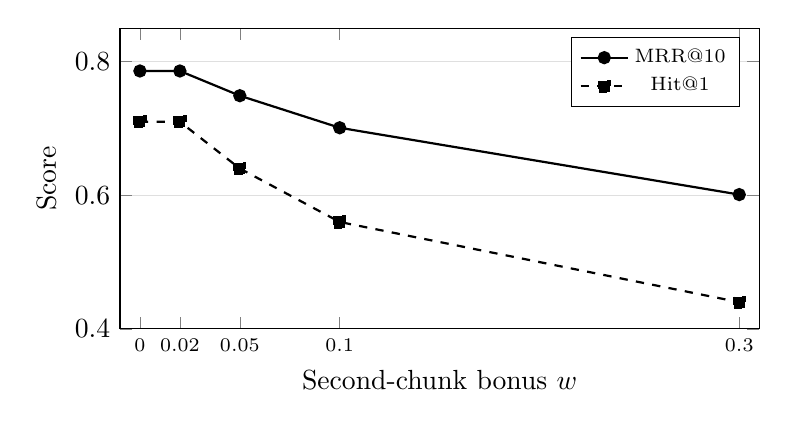
\begin{tikzpicture}
\begin{axis}[
  width=0.8\textwidth, height=5.4cm,
  xlabel={Second-chunk bonus $w$}, ylabel={Score},
  xmin=-0.01, xmax=0.31, ymin=0.4, ymax=0.85,
  xtick={0,0.02,0.05,0.1,0.3}, xticklabel style={font=\scriptsize, /pgf/number format/fixed},
  legend style={font=\scriptsize, at={(0.97,0.97)}, anchor=north east},
  ymajorgrids, grid style={gray!25}, mark size=2pt,
]
\addplot[thick, mark=*] coordinates {(0,0.786) (0.02,0.786) (0.05,0.749) (0.1,0.701) (0.3,0.601)};
\addplot[thick, dashed, mark=square*] coordinates {(0,0.71) (0.02,0.71) (0.05,0.64) (0.1,0.56) (0.3,0.44)};
\legend{MRR@10, Hit@1}
\end{axis}
\end{tikzpicture}
\caption{Effect of the second-chunk bonus on hybrid search}
\label{fig:sweep}
\end{figure}

\section{Other Findings}

\begin{itemize}
  \item \textbf{The relevance floor costs nothing on SciFact.} Removing it
  changed MRR@10 by 0.001 and left no claim without results; it removes
  weak vector-only matches, and the right abstract is rarely one of them. In
  real libraries it is what keeps unrelated pages off short result lists.
  \item \textbf{Hybrid and vector-only are level.} SciFact claims rarely
  share exact words with their abstracts, which favours meaning-based
  search. Hybrid is kept because everyday queries contain names, error
  messages, product codes and sites, which a vector-only search can miss.
  \item \textbf{BM25 gains as much as the others from page grouping.} BM25
  alone rose from MRR@10 0.41 with the bonus to 0.71 without it.
\end{itemize}

\section{Comparison with the Prototype}

\begin{table}[H]
\centering
\small
\begin{tabular}{llccc}
\toprule
\textbf{Version} & \textbf{Configuration} & \textbf{MRR@10} & \textbf{Recall@10} & \textbf{nDCG@10} \\
\midrule
\multirow{3}{*}{Prototype}
 & BM25 only & 0.648 & 0.812 & 0.678 \\
 & Vector only & 0.780 & 0.887 & 0.801 \\
 & Hybrid (min-max) & 0.754 & 0.917 & 0.789 \\
\midrule
\multirow{3}{*}{Final}
 & BM25 only & 0.705 & 0.837 & 0.728 \\
 & Vector only & \textbf{0.812} & \textbf{0.932} & \textbf{0.837} \\
 & Hybrid (RRF) & 0.786 & 0.922 & 0.810 \\
\bottomrule
\end{tabular}
\caption{Prototype and final system on SciFact}
\label{tab:proto-compare}
\end{table}

Every configuration of the final system beats its prototype counterpart on
every metric, the result of the stronger embedding model, smaller
overlapping chunks embedded with titles, rank fusion and best-passage page
scoring.

\section{Evaluation on a Personal Library}

SciFact measures scientific claims, not how people look for pages they have
read. A second evaluation runs on a real library with queries written by its
owner, each labelled \emph{navigational}, \emph{site}, \emph{topic} or
\emph{time}, and reports Recall@1/3/5/10 and MRR per category, with a
compare tool that lists every query whose rank changed. It was used to
measure site, time and URL understanding on a development library of 31
browsed pages among about 1{,}000 SciFact distractors:

\begin{table}[H]
\centering
\small
\begin{tabular}{lcccc}
\toprule
& \multicolumn{2}{c}{\textbf{Right page first}} & \multicolumn{2}{c}{\textbf{MRR}} \\
\cmidrule(lr){2-3}\cmidrule(lr){4-5}
\textbf{Query set} & before & after & before & after \\
\midrule
35 queries used while building & 0.86 & 0.94 & 0.900 & 0.971 \\
18 held-out queries & 0.72 & 0.94 & 0.787 & 0.944 \\
\bottomrule
\end{tabular}
\caption{Effect of site and time understanding on a personal library}
\label{tab:personal}
\end{table}

Most of the gain is in site queries (held-out MRR 0.75 $\rightarrow$ 1.00)
and time queries (0.38 $\rightarrow$ 1.00); topic-only queries are
unaffected, as intended. The sets are small, so the results indicate
direction rather than precise size.
